\documentclass[preprint]{aastex}

\usepackage{natbib,epsfig}
\citestyle{aa}
\usepackage{anysize}

\setlength{\textheight}{9.50in}      % were 23.5/17.9/-2.2/-1.1/1.0cm
\setlength{\textwidth}{6.5in}
\setlength{\topmargin}{-0.25in}      % The ref point is 1" from paper
\setlength{\oddsidemargin}{0.00in}   % edge, top & left.  (Odd/even
\setlength{\evensidemargin}{0.00in}  % margins are for the left side.)
\setlength{\footskip}{0.50in}        % Bottom of body to bottom of foot.

\setlength{\textfloatsep}{0.3in plus 0.1in minus 0.1in}
\setlength{\intextsep}{0.3in plus 0.1in minus 0.1in}
\setlength{\dblfloatsep}{0.3in plus 0.1in minus 0.1in}

\newcommand{\be}{\begin{equation}}
\newcommand{\ee}{\end{equation}}
\newcommand{\ba}{\begin{eqnarray}}
\newcommand{\ea}{\end{eqnarray}}
\newcommand{\bas}{\begin{eqnarray*}}
\newcommand{\eas}{\end{eqnarray*}}

\newcommand{\cnsq}{\ensuremath{C_N{}^{\!2}}}

\usepackage[usenames]{color}

\begin{document}

%\centerline{{\bf{Weak Lensing Section for DES NSF proposal}}}

\section{Weak Lensing: Introduction}

The gravitational bending of light by mass in the universe offers
the opportunity to study the distribution of the dark matter.
Furthermore, lensing measurements of how this distribution
evolves with time and of the distance-redshift relation
tell us about the nature of dark energy.

Due to gravitational lensing, the shapes of distant galaxies will
appear stretched tangentially around a large mass concentration.
Near a massive cluster of galaxies the signal is strong enough to
reconstruct the mass distribution of the object; this is discussed
separately in Section ???. The much weaker, but ubiquitous
signal due to gravitational lensing by the large scale distribution
of mass in the universe, termed ``cosmic shear'', is discussed here.
Several groups published the first detections of this signal
simultaneously in 2000 (Bacon et al. 2000; Van Waerbeke et al. 2000;
Wittman et al. 2000; Kaiser et al. 2000). Since then larger areas of
sky have been analysed, and more sophisticated statistics have been
developed.

The DES will survey an area $30\times$ larger than any current weak
lensing survey.  While this greatly reduces statistical uncertainties,
we must insure that systematic errors in shear measurement, photo-z
determination, and cosmological theory do not come to dominate the
dark-energy error budget.  The DES limits systematic errors to levels
that are verifiable with current data: by using galaxies with $i<24$ for
weak lensing, the typical galaxy size is well resolved by Blanco
imaging, minimizing shape-measurement systematics; the target galaxy
population has well-characterized spectra and colors, and is
accessible to current-data spectroscopic surveys, minimizing photo-z
errors; the requisite theory can be verified with feasible $N$-body
calculations; and the DES performance can be accurately forecast through
analysis of existing data.  Below we enumerate the survey
characteristics relevant to cosmic shear, and the forecasts for DES
performance.

\section{Lensing Statistics}

The primary statistical measure of the cosmic shear
is the shear-shear correlation function or power spectrum.
Since the foreground dark matter is associated to a
large degree with foreground galaxies, one can also measure the
angular cross-correlation between foreground galaxy positions and source
galaxy shear (galaxy-shear correlations, also called galaxy-galaxy
lensing). We will also consider the three-point correlations or
bispectra of the lensing shear.
These weak lensing techniques provide powerful probes of
the dark energy in the context of the Dark Energy Survey. In
addition, as noted in the previous section (???), lensing will provide
statistical cluster mass estimates through the cluster-shear
correlation function that can cross-check SZE and optical richness
mass estimators.

The shear-shear, galaxy-shear, and galaxy-galaxy angular
power spectra can be expressed as projections of the corresponding
three-dimensional power spectra (e.g., Hu \& Jain 2003),
\begin{equation}
C_l^{x_a x_b} = \int dz {H \over D_A^2} W_a(z) W_b(z) P^{s_a s_b}(k=l/D_A;z)\,,
\label{eqn:Limber}
\end{equation}
%where $H(z)$ is the Hubble parameter and
%\begin{eqnarray}
%\langle s_i^*(\bk) s_j(\bk') \rangle &=& (2\pi)^3 \delta(\bk-\bk') P^{s_i s_j}(k
%)\,,
%\end{eqnarray}
%defines the three dimensional source power spectrum.
where $\ell$ denotes the angular multipole, $a, b\in\{1, 2\}$, $x_1$
and $x_2$ denote the two-dimensional angular galaxy (g) and shear
($\gamma$) fields, and $s_1$ and $s_2$ respectively denote the
three-dimensional galaxy (g) and mass (m) density fluctuation fields
at redshift $z$. The weight functions $W_1$ and $W_2$ encode
information about the galaxy redshift distribution and about the
efficiency with which foreground masses shear background galaxies as
a function of their respective distances.

The dark energy density and equation of state affect these angular
power spectra through the Hubble parameter, the angular diameter
distance, the weight factors, and through the redshift- and
scale-dependence of the three-dimensional power spectra $P^{gg},
P^{mm}$, and $P^{gm}$. For a given choice of cosmological
parameters, the shape of the mass power spectrum $P^{mm}$ is well
constrained on large scales by CMB anisotropy data, and
 $P^{mm}$ can be accurately
predicted from $N$-body cosmological simulations down to some mass
scale.  DES will conduct $N$-body simulations of sufficient accuracy
to make the theoretical uncertainties unimportant. 
The power spectra involving galaxies, $P^{gg}$ and
$P^{gm}$, require, in addition to cosmological information, a
model for the bias, that is, for how luminous 
galaxies are distributed with respect to the dark matter. Since
galaxy bias is a complex process, we have based our forecasts on a
conservative analysis that 
%%% ??? Changed the following to more accurately describe gb's approach:
%%marginalizes over 5 free parameters
%%related to bias in each redshift bin (25 bias parameters in all).
%%These parameters are based on the halo occupation distribution model
%%(see Hu \& Jain 2003 for details) that describes how galaxies above
%%some luminosity occupy dark matter halos as a function of halo mass.
%%For the forecasts in Table 1, we use a minimum
%%halo mass of $10^{12.5} M_\odot$. Constraints on these bias
%%parameters come mainly from the galaxy angular power spectrum
%%measurement, since it has the highest signal to noise of the three.
%%This bias model is physically motivated, accurately reproduces the
%%results of N-body simulations that include gas dynamics or that
%%resolve sub-halos, and accounts for the galaxy two-point correlation
%%function measured as a function of luminosity in the SDSS (Zehavi,
%%et al 2004).
allow the bias (and correlation coefficient) between galaxies and
matter to vary with both redshift (at intervals of $\approx 0.05$) and
angular scale (at intervals of $\approx 0.5$~dex).  A sufficiently
accurate model for galaxy bias can significantly improve dark-energy
constraints beyond this simple model where biases are free parameters
({\it e.g.} Hu \& Jain 2003).

To forecast constraints, we estimate the statistical errors on the
angular power spectra; for example, for the shear-shear spectrum,
the uncertainty is (Kaiser 1992)
\begin{equation}
\Delta C_\ell = \sqrt{\frac{2}{(2\ell+1)f_{\rm sky}} }
\left( C_\ell +\frac{\sigma^2(\gamma_i)}{n_{\rm eff}} \right)
\label{eqn:power_error}
\end{equation}
%
where $f_{sky}$ is the fraction of sky area covered by the survey,
$\sigma^2(\gamma_i)$ is the variance in a single component of the
(two-component) shear, and $n_{\rm eff}$ is the effective number
density per steradian of galaxies with well-measured shapes. The first
term in brackets comes from cosmic 
variance, and the second, shot-noise term results from both the
variance in galaxy ellipticities (``shape noise'') and from
shape-measurement errors due to noise in the images. This expression
assumes the shear field is 
Gaussian; although this assumption breaks down at large $\ell$ due
to non-linearity, the non-Gaussian variance is generally masked by
the shape noise term.  At smaller angular scales, the measurement
uncertainties in the power spectrum can be smaller than the
uncertainties in the theoretical prediction produced by baryonic
effects that are unmodelled in pure-gravity $N$-body simulations
(White 2004; Zhan \& Knox 2004; Jing et al. 2006).  These
uncertainties are included in the forecasts below.

{\bf Need a description of the bispectrum statistic here.}

%%% ??? will this be in here ???
We provide estimates of the degradation due to
the non-Gaussian contribution. 

%%Further, in the Table ??? 
%%forecasts, we only use
%%information from multipoles $\ell <1000$, so the maximum spatial
%%wavenumber used is $k \sim 1 h^{-1}$ Mpc at the typical depth of the
%%survey.


\section{Image Quality}
The measurement error on the lensing statistics depends upon the
quality of the shape and shear measurements of galaxies, which in turn
depends upon the noise level and image quality of the survey data.
For weak lensing, the first important image-quality metric is the
seeing, or PSF {\em size}, which---along with the depth of
  exposures---determines the effective sky density $n_{\rm eff}$ of
  galaxies whose shapes (ellipticities) are sufficiently well measured
  to be useful for cosmic shear.
Another essential metric is the
PSF {\em anisotropy}, usually quantified by its ellipticity, which
  can, if incompletely corrected, be confused with lensing distortions
  of galaxies.  The PSF anisotropy can be divided into a static
  spatial pattern over the field of view, and a time-variable
  component of the PSF pattern.
The static pattern is easily diagnosed using the many thousands of stellar
sources imaged every night, but the time-varying components can be
more problematic, depending upon their angular and temporal scales of
variability. 
We conservatively base all our cosmological forecasts on the current
delivered image quality of the Blanco. Many improvements are being
made, however, to improve this performance beyond
our current predictions, as detailed below.

\subsection{Seeing and Galaxy Density}
The empirical
shape noise for large, well-measured galaxy images is
$\sigma^2(\gamma_i)=(0.16)^2$ (Sheldon et al 2004, Jarvis et al 2003).  Note
that this per-galaxy noise level increases for deeper surveys (ref CFHLS???).
To estimate the $n_{\rm eff}$ for the DES, we study images taken
by the GOODS survey (Dickinson et al. 2003) artificially degraded to different
seeing and noise values.  In addition, a 900 sec CFH12K $I$-band
exposure taken in median seeing of 0.63'' is used for comparison. 
The depth of this image is well-matched to the DES $i$-band
survey requirement, and is thus a good reference point for
the simulation. We first convolve the GOODS images with a gaussian
PSF and then add noise appropriate for DES images.
We measure the ellipticities and sizes of the detected
objects using an adaptive weighting scheme that is nearly optimal for
lensing measurements (Bernstein \& Jarvis 2002). 
The mean weight per galaxy drops from unity
for $I_{AB}\le21.5$ to about 0.5 at $I_{AB}=24.1,$ which is the
nominal $10\sigma$ detection level for galaxies, as the poorer
resolution and higher measurement noise take their toll on the
fainter, smaller galaxies. We have verified that for a seeing
of 0.63'' we recover the effective density of the reference image.

The effective source density for the DES $i$-band images is shown by the lower
line in Fig. \ref{fig:neff_seeing}, as a function of seeing. An increase in
seeing has two effects: (i) the PSF is a larger fraction of the size of the
faint source galaxies, so they receive less weight due to the larger PSF
dilution factor; (ii) the effective number of CCD pixels per object is larger,
increasing the sky background per object and therefore the shape measurement
error.  The upper line assumes that the $r$, $i$ and $z$ bands can be combined
with equal efficacy (integrated exposure times of 400 s in $r$, 1200 s in $i$,
2000 s in $z$) to reduce photon noise and increase the effective number density
of galaxies.  Taking the {\em current} median seeing of 0\farcs9 for the
Blanco/Mosaic imager,
%%% Is this true ???
we adopt an effective source galaxy density of $n_{\rm eff} =12$ arcmin$^{-2}$
for analysis of the DES WL performance.

\begin{figure}[h]
\centerline{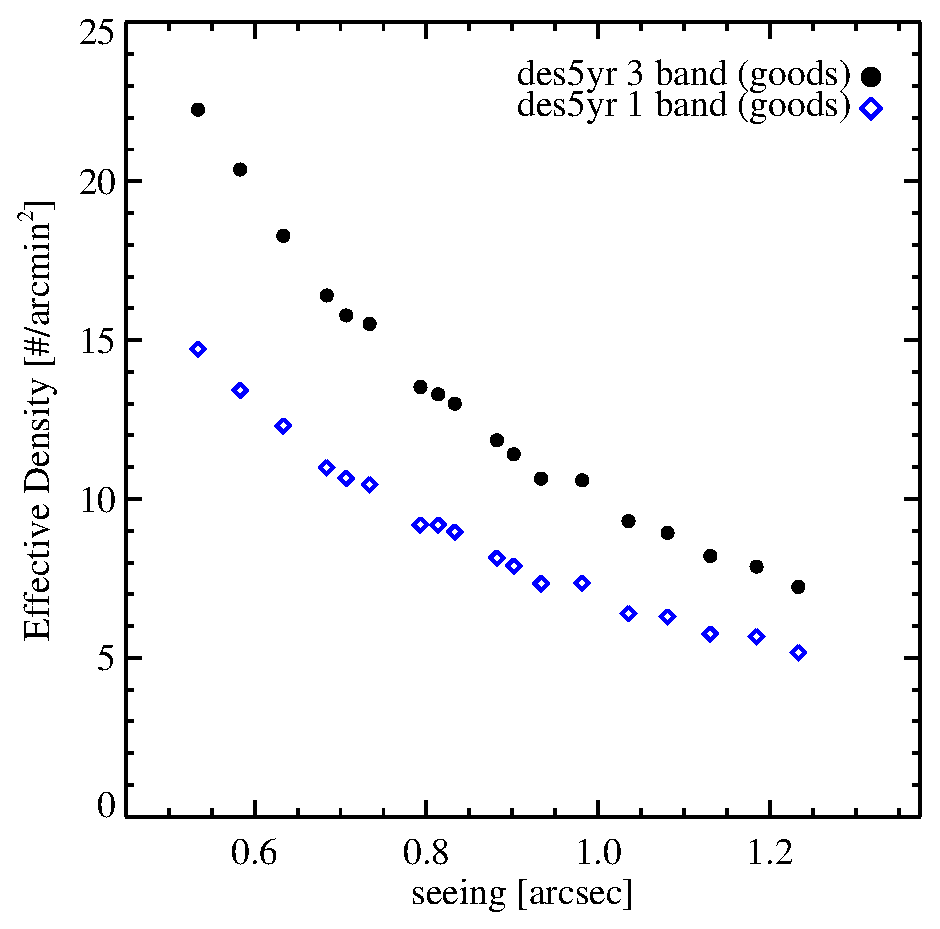
\epsfig{file=des_seeing.eps,width=8cm,angle=0}}
  \caption{
Effective source galaxy density for lensing as function of seeing.
The lower line uses just $i$-band observations and the upper line assumes
that the $r$, $i$ and $z$ bands are combined.
  }
  \label{fig:neff_seeing}
\end{figure}


We find that $n_{\rm eff}$ increases by approximately 17\% per 0\farcs1
reduction in seeing around our fiducial seeing value, so the expected
improvement in Blanco image quality upon installation of DES optics
and feedback systems will modestly improve the dark-energy
constraints.

Note that this {\em effective} source density
is smaller by about a factor of two than the {\em total} density
of sources above the DES 10-$\sigma$ detection limit of the Survey,
because it includes down-weighting due to finite measurement error,
PSF dilution, and shear polarizability.

Finally, we
note that the galaxy-shear correlation function has been measured
with high signal to noise in the SDSS (Sheldon, etal 2004), with
typical seeing of 1.5'' and source density of only $n_{\rm eff} \sim 1$
per square arcmin. By comparison, the DES will cover a similar area
on the sky but go considerably deeper with substantially better
seeing.
%%%%%%%

{\bf Need to look at the text from Brenna about the plans for the
optics}

\subsection{PSF and Distortion Variation}
The dominant shape measurement error in current lensing surveys is
due to the anisotropy of the point spread function (PSF), caused by
optical and CCD distortions, tracking errors, wind shake,
atmospheric refraction, etc. In a given exposure, the PSF anisotropy
is measured using the stars in the field and interpolated to the
positions of the galaxies. Because the density of stars is
relatively low, the errors in this interpolation can lead to
significant coherent errors in the measured shapes of galaxies that
are difficult to distinguish from the lensing shear. This leads to
additive errors in the shear that must either be eliminated or
marginalized over. Since the PSF anisotropy depends on the detailed
optical-mechanical properties of a telescope as well as observing
conditions, it is specific to each telescope and observing site. The
error in measuring the PSF anisotropy can be reduced by combining
data from multiple pointings of a telescope, increasing the
effective density of stars. However, time variability of the PSF
shapes limits the effectiveness of this technique. Recently the
error in measuring the PSF shape has been substantially reduced by
introducing a Principal Component Analysis (PCA) technique that
optimally uses information on the PSF from multiple exposures
(Jarvis \& Jain 2004); this enables interpolation of the PSF with
much finer effective angular resolution. This is especially
promising for the DES, since it has already been applied to data
taken with the BTC and Mosaic II imagers on the Blanco telescope.

We have examined the principal components of the distortion patterns
of data from the existing Blanco optics and made forecasts for how
well the DES could correct these. 
%%Can we omit this: From the current design for the DES optical corrector
We expect the level of raw PSF anisotropy to be a few
percent. Subtraction of the static pattern reduces
this to the percent level(???), and we have estimated that with the PCA
technique we will be able to reduce it further by over a
factor of 100. This is based on the analysis of Jarvis \& Jain
(2004) and Jain, Jarvis \& Bernstein (2006), 
scaled conservatively to the number of exposures for DES
(the correction improves with the number of exposures). In this
extrapolation we have accounted for the number of well-measured
stars available to estimate the principal components. The estimated
residuals are well below the statistical errors. Hence we believe
that additive errors in the estimated shear due to time-varying PSF
patterns will be negligible in
the error budget of DES lensing measurements.

To improve the optical quality and stability of the Blanco, 
we have begun a detailed
analysis of the optical distortions of the Blanco using ray tracing
to model imaging data taken with the Mosaic II and BTC cameras. We
have tentatively identified the dominant distortion patterns
empirically measured by Jarvis \& Jain (2004) with focusing errors
(coupled to astigmatism in the primary mirror), misalignments or
tilts between the primary mirror and the optical axis defined by the
camera and corrector (inducing coma), guiding errors, and trefoil
distortions of the primary mirror associated with its support
system.
DECam is being designed and the telescope upgraded and enhanced to
reduce or eliminate these systematic effects. The reference DECam
optical corrector design achieves small and smoothly varying PSF
distortions across the field of view, with an amplitude comparable
to other recent or planned wide field optical correctors.  DECam
will be equipped with dedicated CCDs, absent from the Mosaic II,
to provide continuous active control of the focus. %%% true???
The reference DECam optical corrector design does not
include an atmospheric dispersion compensator (ADC), eliminating one
source of coma. At present we are considering incorporating wave
front sensors along with two-axis motions of the prime focus cage to
actively recollimate the telescope during the night (see Section 8).
The telescope is also being instrumented with position monitors to
better understand the performance of the primary mirror support
system and flexure of the telescope truss.  Broken radial supports
on the primary mirror have long been a source of difficulty, but the
causes have been identified and a new design for attaching the
rebalanced supports to the mirror is being studied and should
resolve this problem.

\begin{figure}[h]
\centerline{}
  \caption{
Predicted PSF pattern from an optical model of the existing
Blanco corrector, with the primary mirror offset by 0.2 mm in $x$ and
-0.7 mm in $y$ from the optical axis. In situ measurements have
indicated the presence of time-dependent offsets of this magnitude,
likely due to failure of some of the primary mirror radial supports.
The inscribed box shows the area covered by the Mosaic II CCDs. The
offset introduces coma in addition to that induced by the
atmospheric dispersion compensator (ADC). This pattern is
qualitatively similar to some PSF distortion patterns seen with the
Mosaic II imager.
  }
  \label{fig:model_seeing}
\end{figure}

\section{Cosmological Constraints}

We have computed the Fisher forecasts for dark energy parameters
feasible with lensing measurements with DES using multiple statistics
and the levels of measurement error conservatively estimated above for
the DES noise level and image quality. While the primary
lensing statistic for cosmological constraints is the shear power
spectrum (measured in multiple 
redshift bins), we also use the galaxy-shear power spectrum,  plus
the bispectrum (for $\ell<1000$).

For the bispectrum forecast, we have combined information from
triangles of all configurations and tomographic bins (Takada \& Jain
2004). By the time of the survey, we intend to verify the analytical
methods used here with ray tracing simulations. In particular we
will include various higher order effects (Dodelson \& Zhang 2005)
and the non-Gaussian covariance between the power spectrum and
bispectrum; initial results indicate that the impact on parameter
constraints will be significant. The covariance between the power
spectrum and bispectrum at $\ell$ below 1000 degrades parameter errors
by no more than ???\%(e.g. Kilbinger \& Schneider 2005; Takada \&
Jain, in preparation). 


\subsection{Systematic errors} \label{sec:systematics}

Because weak lensing is a subtle effect and the DES will have a
statistical noise well below current data, it is essential to include
the effect of potential systematic errors on the constraints. 
Systematic errors in weak lensing measurements can arise from:
incorrect shape measurements; biases in the photometric redshifts
of galaxies; intrinsic correlations of galaxy shapes; and inaccuracies
in predictions of nonlinear structure growth. The DES experimental
design minimizes the size of these systematics and their effect on
dark-energy determination {\color{red} XXX not intrinsic}.

Shape measurement errors result from incorrect
calibration or errors in correction of the anisotropic point spread
function (PSF) and lead to erroneous multiplicative or additive
factors in the estimated lensing shear, respectively. The lensing
shear we wish to measure is ~1\% on arcminute scales and drops to
~0.1\% on degree scales; the goal is to reduce the sum of all
systematic errors below statistical errors over at least this range
of angular scales.

Given the subtle nature of lensing systematics and the novelty of
analysis techniques in this field, the DES is a low-risk survey
because it is relatively shallow and the Blanco telescope is well
studied. The shallow depth of the survey means the lensing signal
will be lower, but more importantly, the relatively large angular sizes
(compared to the seeing disk) of the
source galaxy population will simplify considerably the correction
of systematic errors. Given the typical delivered seeing at the
Blanco, the depth versus area trade-off of DES is well suited for
obtaining the best possible lensing measurements. The 75 square
degree lensing survey of Jarvis et al (2005) using the Blanco
telescope has comparable depth to DES in the $r$-band; their results
demonstrate the feasibility of the planned measurements with DES.

The relatively shallow survey of DES also minimizes systematic errors
in photometric redshifts, since a spectroscopic survey calibrating the
photo-z's can feasibly sample the full population used in the lensing
analysis. There will be no need to extrapolate the spectral behavior
of galaxies to magnitudes or galaxy types that are too faint for
spectroscopy. 

The DES will gather dark-energy information from galaxy-galaxy
correlations, galaxy-shear correlations, and shear-shear
correlations.  Shear-shear correlations are completely independent of
the bias model for galaxies but subject to additive and
multiplicative shear systematics.
Galaxy-shear correlations are somewhat dependent on galaxy theory, but
are insensitive to additive shear systematics because these are
uncorrelated with the galaxy distribution.  And galaxy-galaxy
correlations are of course insensitive to any shear systematics, but
more dependent on the halo occupation prescription.  This variety of
statistics with distinct systematic susceptibilities permits a robust
determination of dark energy.

\subsection{Systematic errors: shear calibration}
As noted above, we have calculated the expected additive shear error
due to time-varying PSF ellipticity patterns, and find that the PCA
technique should reduce them to negligible levels.  
A second kind of shape measurement error arises due to calibration
errors and contributes a multiplicative term to the shear; it can
arise, for example, from inaccurate correction for the circular
blurring of galaxy images (and consequent reduction in ellipticity)
due to seeing. It is reassuring that calibration errors appear to be the
least dangerous systematic for cosmological measurements (Huterer et
al 2005). Unlike additive errors, with calibration errors there is
less freedom in mimicking the redshift dependence of the signal.
Hence even if the calibration errors increase from 0.4\% to 4\% of
the shear, Fig. 3.1 shows that the resulting constraint on $w$
degrades by less than a factor of two. Moreover, the shear
measurements can be studied as a function of source galaxy angular
size; since the calibration uncertainties go down as the square of
the PSF divided by galaxy size, the consistency of the shear signal
as a function of source galaxy size provides a check on these
calibration errors.

The finite size of the PSF and the distribution of
intrinsic shapes of galaxies need to be accurately measured to
calibrate the shear. This has been done in recent studies by a
careful combination of analytical techniques and tests with
simulated images. Initial results from an ongoing set of tests known
as the STEP program (Heymans et al 2005) and from Nakajima \&
Bernstein (2006) suggest that software based
on the Bernstein \& Jarvis (2002) approach can achieve a calibration
accuracy approaching the requirements for DES.  

More specifically, the
Fisher forecasts below assume that each bin of width 15\% in $(1+z)$
has an independent shear calibration factor that is unknown and must
be marginalized when deriving dark-energy parameters.  We assume that
the prior knowledge of these calibration factors has an RMS
uncertainty of 0.01 per bin.  Nakajima \& Bernstein (2006) demonstrate
a shear recovery technique that reaches accuracy of 1\% or better over
a range of noise and resolution levels that span those to be expected
in the DES data.  These results must be validated with more extensive
tests during the DES simulations, and refinement of the methods will
likely allow a more aggressive prior to be assumed for the shear
calibration errors.

{\bf Figure 3}  Degradation in error on cosmological parameters due to
marginalizing over uncorrected multiplicative shear systematic
errors, from Huterer et al. (2005).

\subsection{Systematic errors: photometric redshifts}

The impact of systematic photometric redshift errors on shear-shear
measurements in the DES have been studied by Huterer, et al. (2005)
and by Ma, Hu, \& Huterer (2005). 
For source galaxies binned by photometric redshift, they find
that the error (bias) in the centroids of the photo-z bins must be
measured at the level of 0.002 or less and the scatter in the
photo-z errors per bin known to an accuracy better than 0.01 in
order to keep the lensing constraint on $w$ from degrading by more
than 10\%. Using a subsample of galaxies with measured spectroscopic
redshifts, the photo-z error distribution as a function of redshift
can be measured, and this scatter and bias inferred, with an
uncertainty depending on the size of the spectroscopic sample. For
the characteristic photo-z errors predicted by the DES photo-z
simulations described in Section ???, Ma, Hu, \& Huterer (2005) show
that a spectroscopic training set that reaches the DES
photometric depth and comprises 50,000-100,000 galaxy redshifts will
achieve these desired accuracies. As noted in Section ???, on-going
deep spectroscopic surveys will provide such a sample before DES
begins taking data, and we therefore expect photo-z systematic
errors to be under control for DES weak lensing.

\subsection{Systematic errors: intrinsic alignments}

Any tendency of galaxies to align with their neighbors---or to align
with the local mass distribution---can be confused with alignments
caused by foreground gravitational lensing, thus biasing dark-energy
determinations.  It is, however, possible to distinguish intrinsic
alignments from true lensing once photometric redshift information is
available for all source galaxies, because these effects have distinct
redshift dependencies.  Table (Figure) ??? illustrates that, for
DES-quality data, one can solve for lensing and intrinsic alignments 
simultaneously with modest degradation of dark-energy constraints if
different lensing statistics are combined. 

\subsection{Systematic errors: theory uncertainty}

At sufficiently large angular scales, the matter distribution evolves
under linear perturbation theory and the lensing signal is calculable
to high accuracy for a given dark-energy model.  At smaller scales,
$N$-body simulations of gravitational growth are required to predict
the signal.  The DES project will excecute numerical simulations
sufficiently accurate to exploit its weak lensing data.
At still smaller scales, baryonic effects become important and are
more difficult to simulate.  Our weak lensing forecasts include the
uncertainties that are expected to arise from baryonic effects
(White 2004, Zhan \& Knox 2004, Jing et al. 2006), and the degradation
to dark-energy constraints is minor. 

\subsection{Results}
Plot the Fisher results here...

\section{Weak lensing constraints on clusters}

% Added by E.S.
The use of galaxy clusters to constrain Dark Energy requires knowledge of their
masses.  For example, the method of the SPT SZE survey involves counting the
number of clusters above a fixed mass threshold as a function of redshift.  The
SZE Y-parameter is a measure of the pressure in the cluster. It is expected
that Y is tightly correlated with mass, but this correlation must be measured
separately or marginalized over.

Weak lensing will be used to constrain the mass-observable relationship in the
DES/SPT.  The DES is deep enough to constrain the masses of individual clusters
over a certain range of masses and redshifts.  Also, the averaged signal, the
cluster-shear correlation function, can be measured with high precision over a
larger range of masses and redshifts (Sheldon et al. 2007).  This average
signal is the more desirable method as it is simpler to interpret and free of
certain systematics (e.g. additive shear errors. See \S \ref{sec:systematics})
and noise (e.g.  structures along the line of sight).

The cluster mass-luminosity relationship has been measured to 10\% statistical
error over a factor of $10^3$ in mass in the relatively shallow Sloan Digital
Sky Survey (Sheldon et al. 2007, Johnston et al. 2007).  The shallow SDSS
survey has a factor of 12 smaller effective source density than the DES, and
the signal from the low redshift lenses and sources is many times smaller than
that in the DES.  Furthermore, the larger volume surveyed by DES will yield a
larger number of high mass objects and allow the mass-observable relationship
to be tracked as a function of redshift.  Thus, we will constrain the
mass-observable relation to a few percent in redshift slices of equal volume
to the SDSS.

{\color{red} XXX good enough, or should we run numbers for some redshift bins?.
For example, how many effective SDSS volumes will we get given that higher
redshift sources get downweighted?  }

\end{document}

